\documentclass[10pt]{beamer}

\usetheme{metropolis}
\usepackage[export]{adjustbox}
\usepackage[french]{babel}
\usepackage[scale=2]{ccicons}
\usepackage[utf8]{inputenc}
\usepackage{appendixnumberbeamer}
\usepackage{booktabs}
\usepackage{colortbl} 
\usepackage{graphicx}
\usepackage{hyperref}
\usepackage{longtable}
\usepackage{multicol}
\usepackage{multirow}
\usepackage{pgfplots}
\usepackage{pifont}
\usepackage{smartdiagram}
\usepackage{subcaption}
\usepackage{tabularx}
\usepackage{tikz}
\usepackage{url}
\usepackage{wrapfig}
\usepackage{xcolor}
\usepgfplotslibrary{dateplot}
\usesmartdiagramlibrary{additions}
%\usetheme[progressbar=frametitle]{metropolis}
%\usepackage{biblatex}
%\usepackage{natbib}

\usepackage{xspace}
\newcommand{\themename}{\textbf{\textsc{metropolis}}\xspace}

\title{Introduction : Le numérique au service des Humanités \dots et vice-versa} %Traiter automatiquement les données textuelles dans le contexte des Humanités : quelques exemples}
%Observables in an NLP pipeline : Virtues and Flaws of the reductionist approach}
%\subtitle{A modern beamer theme}
\date{1 Octobre 2026}
\author{Gaël Lejeune (gael.lejeune@sorbonne-universite.fr)}
\institute{
	UFR de Sociologie et d'Informatique pour les Sciences Humaines\\
	STIH, Sorbonne Université\\
           CERES~(Expérimentations en Méthodes numériques pour les SHS)
}
 \titlegraphic{
\hfill
\includegraphics[height=1cm]{Images/1.png}
\hfill
\includegraphics[height=1.2cm]{Images/STIH.png}
\hfill
\includegraphics[height=1cm]{Images/sorbonne.png}
\hfill
\includegraphics[height=1.2cm]{Images/logo-dimeco.png}
\hfill
}
\usepackage{array}
\begin{document}

\maketitle


\begin{frame}{Qui suis-je}

	\begin{block}{Parcours universitaire}
\begin{itemize}
  \item L: Sciences du Langage (Caen)
  \item M: Traductologie (Caen, Corfou, Helsinki)
\pause
  \item D: Informatique (Caen)
\pause
  \item puis Nantes, Paris XIII, Sorbonne Université
\end{itemize}
	\end{block}
\pause

	Spécialité : \textbf{Traitement Automatique des Langues}

	\begin{block}{Champs d'application}
\begin{itemize}
  \item Veille Epidémiologique et Extraction d'Info  Multilingue
\pause
  \item Classification de Documents (dialectes, opinions \dots)
\pause
  \item Analyse Stylistique (auteurs, dates, genres \dots)
\pause
  \item Analyse de Réseaux Soc. Numériques
\end{itemize}
	\end{block}
\end{frame}


\begin{frame}{Ce dont je vais parler ici}

\begin{itemize}
%  \item Traitement Automatique des Langues (TAL) VS analyse des Données Textuelles (ADT), cf. M.Valette JADT 2016
%\pause
  \item Magie de l'outil automatique et pyrotechnie formelle
\pause
  \item Les Humanités comme objet d'application  du numérique \pause
  \item \dots et comme objet de réflexion sur le numérique
\pause
  \item Cadre : Centre d'Expérimentation des Méthodes Numériques en SHS
\end{itemize}
	\begin{block}{Domaines mobilisés} 
\begin{itemize}
\item Traitement Automatique des Langues (TAL)
\item Vision par Ordinateur
\item Fouille de Données
\end{itemize}
\end{block}

\end{frame}

\begin{frame}{Organisation}
	Des cours de 2h  (masi probablement pas 13) :
%TODO: Changer pour M2
\begin{itemize}
\item Du bla-bla \dots  puis De la pratique
\pause
 \item De la réflexion 
\pause
 et encore De la pratique
\end{itemize}
%TODO: Changer pour M2
%Evaluation : peut-on outiller votre sujet de mémoire ? A quel moment ?

%DMT

%TODO : CRS

\end{frame}

\begin{frame}{Outline}
  \setbeamertemplate{section in toc}[sections numbered]
  \tableofcontents[hideallsubsections]
\end{frame}

\section{Acteurs des Humanités Numériques : Le CERES} %, Humanités Numériques à l'Université}

\pause
\begin{frame}{CERES}
  Centre d'Expérimentation pour les \textbf{Méthodes Numériques} en SHS
\begin{itemize}
  \item Contexte : Faculté des Lettres de SU
  \pause
  \item Pas ou peu d'ingénieurs de recherche
  \item Mais de nombreuses disciplines (sauf droit)
  \pause
  \item Le numérique entre espérance et méfiance
\end{itemize}
\end{frame}

\begin{frame}{CERES en un slide}

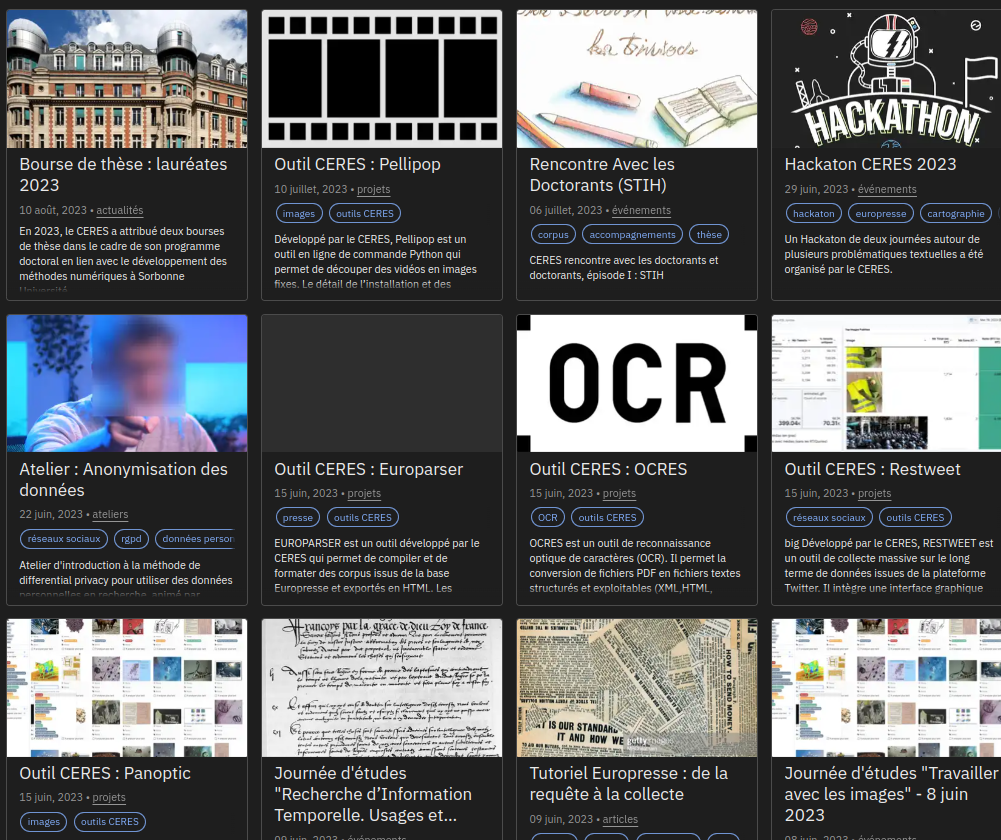
\includegraphics[width=.9\textwidth]{Images/toto.png}
\end{frame}

\section{Partie 1 : Traiter des données textuelles}

\begin{frame}{Les termes du débat}

%%	Approches \textbf{tout-terrain ou ad hoc} :
%%comment concevoir des applications de TAL
%%	\textbf{robustes} à la \textbf{variation} dans les données?
%%
%%	\begin{block}{Eléments de comparaison}
%%\begin{itemize}
%%  \item Ad hoc VS tout-terrain
%%  \pause
%%  \item Robuste VS \dots
%%  \pause
%%  \item Variation VS \dots
%%\end{itemize}
%%\end{block}
%%\pause
	Une application "numérique:
\begin{itemize}
  \item des données
  \item des tâches
\pause
  \item des méthodes
\end{itemize}

\pause
Si Données = Texte,

\pause
Et si Tâches = (Moteur de Recherche, Traduction, Génération \dots)

\pause
Alors la Méthode a à voir avec le Traitement Automatique des Langues

\end{frame}

\begin{frame}{Le Traitement Automatique des Langues par l'exemple}
\begin{figure}
 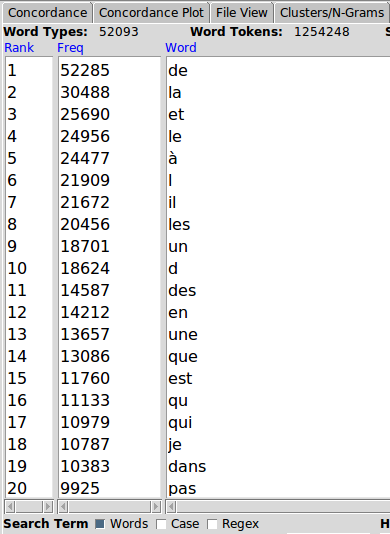
\includegraphics[width=.5\textwidth]{Images/TAL/01_WordList.png}
	\caption{Trouver les mots les plus fréquents (Antconc \cite{anthony2020antconc})}
\end{figure}
\end{frame}

\begin{frame}{Focus: Traitement Automatique des Langues}
\begin{figure}
 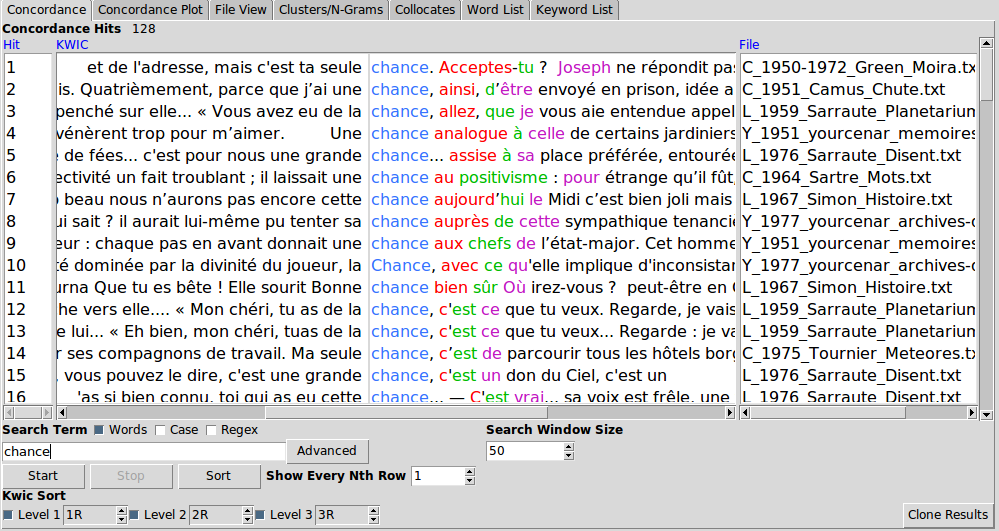
\includegraphics[width=.8\textwidth]{Images/TAL/02_Concordance.png}
\caption{Un mot en contexte  (Antconc)}
\end{figure}
\end{frame}

\begin{frame}{Focus: Traitement Automatique des Langues}
\begin{figure}
 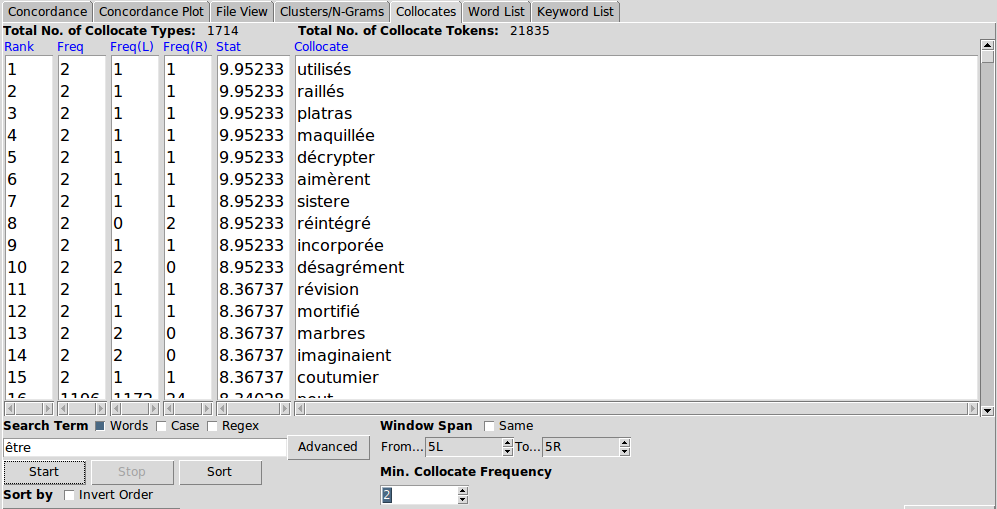
\includegraphics[width=.8\textwidth]{Images/TAL/03_Collocations_Antconc.png}
\caption{Les co-occurrents d'un mot (Antconc)}
\end{figure}
\end{frame}

\begin{frame}{Focus: Traitement Automatique des Langues}
\begin{figure}
 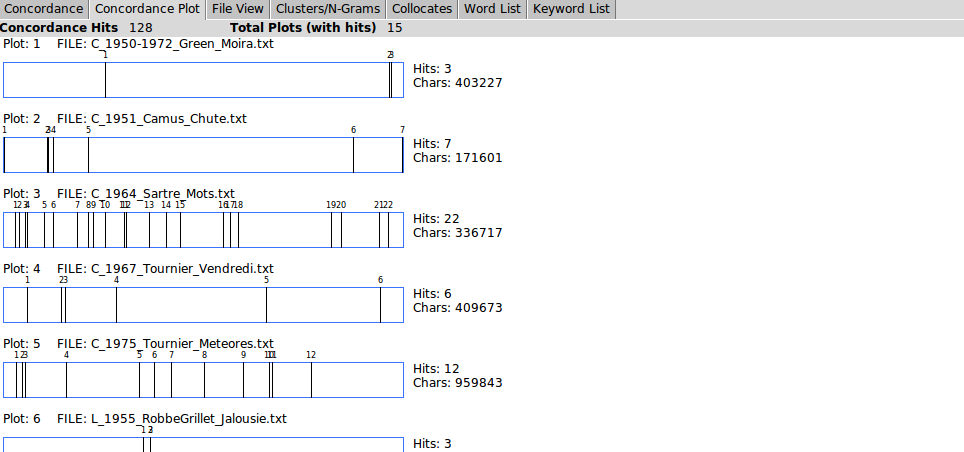
\includegraphics[width=.8\textwidth]{Images/TAL/04_ConcordancePlot.png}
\caption{Voir un mot au fil de différentes œuvres}
\end{figure}
\end{frame}

\begin{frame}{Focus: Traitement Automatique des Langues}
\begin{figure}
 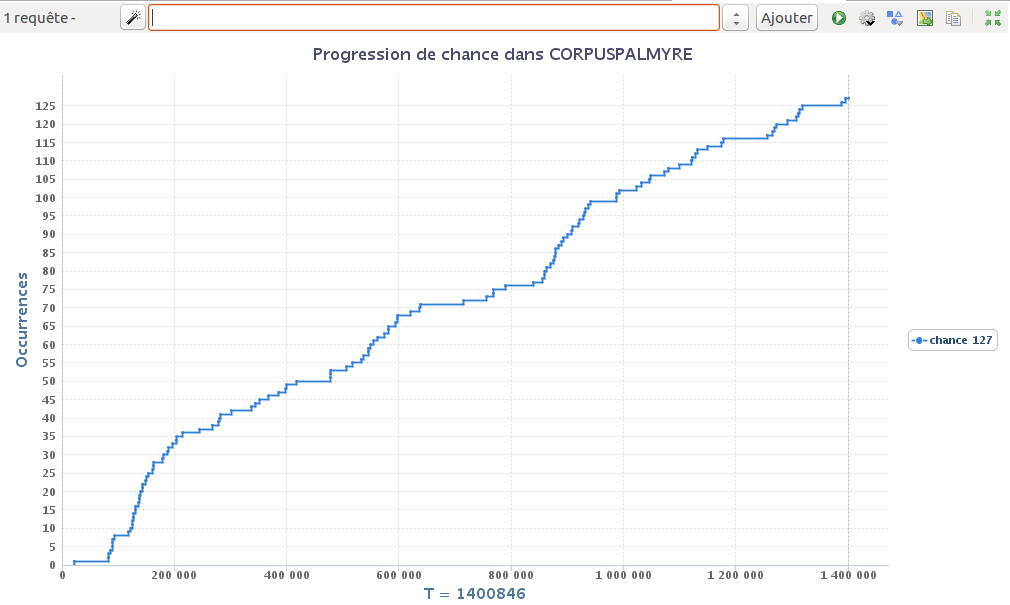
\includegraphics[width=.8\textwidth]{Images/TAL/05_Progression_TXM.png}
	\caption{La progression de la fréquence d'un mot dans le temps (TXM \cite{heiden2010txm})}
\end{figure}
\end{frame}

\begin{frame}{Focus: Traitement Automatique des Langues}
\begin{figure}
 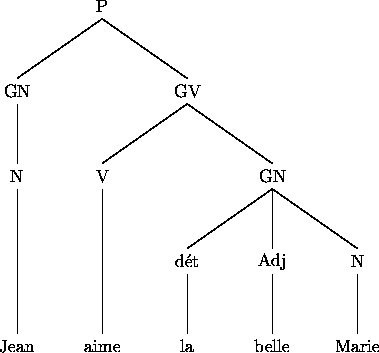
\includegraphics[width=.6\textwidth]{Images/TAL/06_analysesyntaxique.png}
\caption{Représentation Syntaxique d'une Phrase}
\end{figure}
\end{frame}

\begin{frame}{Focus: Traitement Automatique des Langues}
\begin{figure}
 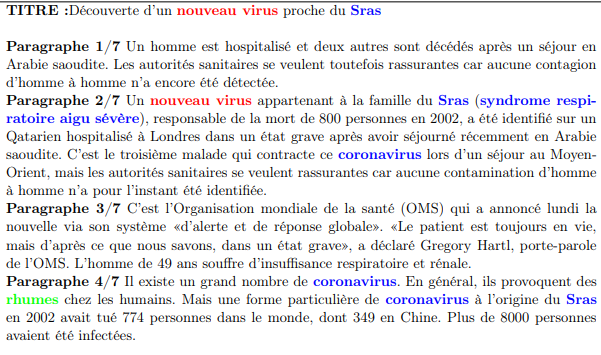
\includegraphics[width=.8\textwidth]{Images/TAL/07_EI_daniel.png}
	\caption{Extraction d'Information (Daniel \cite{Lejeune-2013_These})}
\end{figure}
\end{frame}

\begin{frame}{Focus: Traitement Automatique des Langues}
\begin{figure}
 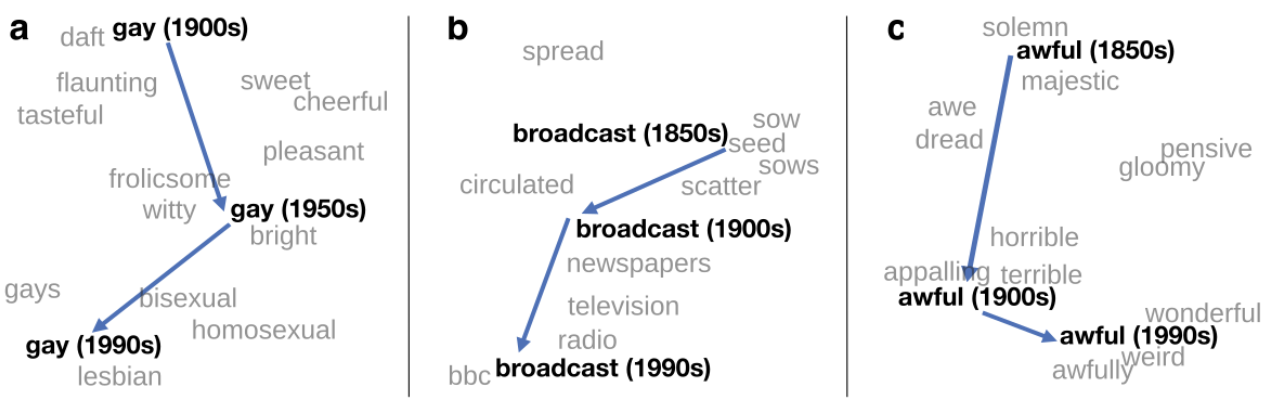
\includegraphics[width=.8\textwidth]{Images/TAL/08_semantic_change.png}
	\caption{Changement Sémantique (Dan Jurafsky \cite{hamilton2016diachronic})}
\end{figure}
\end{frame}

\begin{frame}{Focus: Traitement Automatique des Langues}
\begin{figure}
 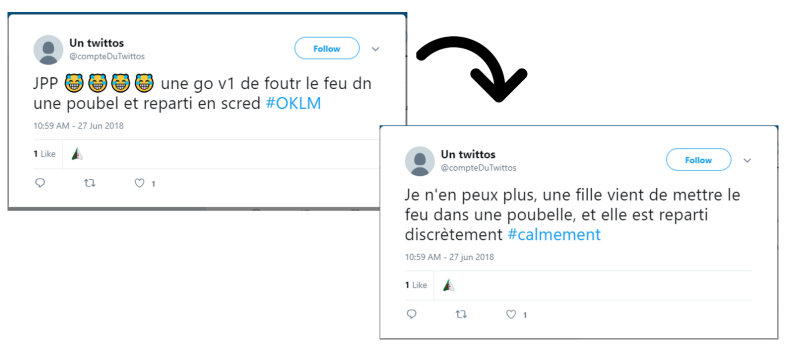
\includegraphics[width=.8\textwidth]{Images/TAL/09_twitter_47.png}
\caption{Traduction et "Standardisation"}
\end{figure}


\end{frame}

\begin{frame}{Conditions de réalisation de statistiques sur du texte}
 \pause
\begin{itemize}
  \item Des données
  \item Représentatives
  \item Dans un format approprié
  \item En un mot : un \textbf{corpus} !
\end{itemize}

	%\pause

%Sur quel corpus travaillez vous pour votre mémoire ?

%Avec quel objectif ?

%https://docs.google.com/spreadsheets/d/1V6-VTm8kfBJEbtdgOMhpHepuL38OhJjtVGTQuzE9TQ8/edit?gid=0#gid=0

\end{frame}

%%\begin{frame}[allowframebreaks]{References}
%%	\footnotesize{
%%  \bibliography{biblio}
%%  \bibliographystyle{apalike}
%%	}
%%\end{frame}
\end{document}

